%
% This is a borrowed LaTeX template file for lecture notes for CS267,
% Applications of Parallel Computing, UCBerkeley EECS Department.
% Now being used for CMU's 10725 Fall 2012 Optimization course
% taught by Geoff Gordon and Ryan Tibshirani.  When preparing 
% LaTeX notes for this class, please use this template.
%
% To familiarize yourself with this template, the body contains
% some examples of its use.  Look them over.  Then you can
% run LaTeX on this file.  After you have LaTeXed this file then
% you can look over the result either by printing it out with
% dvips or using xdvi. "pdflatex template.tex" should also work.
%

\documentclass[twoside]{article}
\setlength{\oddsidemargin}{0.25 in}
\setlength{\evensidemargin}{-0.25 in}
\setlength{\topmargin}{-0.6 in}
\setlength{\textwidth}{6.5 in}
\setlength{\textheight}{8.5 in}
\setlength{\headsep}{0.75 in}
\setlength{\parindent}{0 in}
\setlength{\parskip}{0.1 in}

%
% ADD PACKAGES here:
%

\usepackage{amsmath,amsfonts,graphicx}

%
% The following commands set up the lecnum (lecture number)
% counter and make various numbering schemes work relative
% to the lecture number.
%
\newcounter{lecnum}
\renewcommand{\thepage}{\thelecnum-\arabic{page}}
\renewcommand{\thesection}{\thelecnum.\arabic{section}}
\renewcommand{\theequation}{\thelecnum.\arabic{equation}}
\renewcommand{\thefigure}{\thelecnum.\arabic{figure}}
\renewcommand{\thetable}{\thelecnum.\arabic{table}}

%
% The following macro is used to generate the header.
%
\newcommand{\lecture}[4]{
   \pagestyle{myheadings}
   \thispagestyle{plain}
   \newpage
   \setcounter{lecnum}{#1}
   \setcounter{page}{1}
   \noindent
   \begin{center}
   \framebox{
      \vbox{\vspace{2mm}
    \hbox to 6.28in { {\bf EE302 - Feedback Systems
	\hfill Spring 2019} }
       \vspace{4mm}
       \hbox to 6.28in { {\Large \hfill Lecture #1 \hfill} }
       \vspace{2mm}
       \hbox to 6.28in { {\it Lecturer: #2 \hfill } }
      \vspace{2mm}}
   }
   \end{center}
   \markboth{Lecture #1}{Lecture #1}

   \vspace*{4mm}
}
%
% Convention for citations is authors' initials followed by the year.
% For example, to cite a paper by Leighton and Maggs you would type
% \cite{LM89}, and to cite a paper by Strassen you would type \cite{S69}.
% (To avoid bibliography problems, for now we redefine the \cite command.)
% Also commands that create a suitable format for the reference list.
\renewcommand{\cite}[1]{[#1]}
\def\beginrefs{\begin{list}%
        {[\arabic{equation}]}{\usecounter{equation}
         \setlength{\leftmargin}{2.0truecm}\setlength{\labelsep}{0.4truecm}%
u         \setlength{\labelwidth}{1.6truecm}}}
\def\endrefs{\end{list}}
\def\bibentry#1{\item[\hbox{[#1]}]}

%Use this command for a figure; it puts a figure in wherever you want it.
%usage: \fig{NUMBER}{SPACE-IN-INCHES}{CAPTION}
\newcommand{\fig}[3]{
			\vspace{#2}
			\begin{center}
			Figure \thelecnum.#1:~#3
			\end{center}
	}
% Use these for theorems, lemmas, proofs, etc.
\newtheorem{theorem}{Theorem}[lecnum]
\newtheorem{lemma}[theorem]{Lemma}
\newtheorem{proposition}[theorem]{Proposition}
\newtheorem{claim}[theorem]{Claim}
\newtheorem{corollary}[theorem]{Corollary}
\newtheorem{definition}[theorem]{Definition}
\newenvironment{proof}{{\bf Proof:}}{\hfill\rule{2mm}{2mm}}

% **** IF YOU WANT TO DEFINE ADDITIONAL MACROS FOR YOURSELF, PUT THEM HERE:

\begin{document}

% Lecture Details
\lecture{2}{Asst. Prof. M. Mert Ankarali}

\par

\section*{Conversion Between Different LTI Representations}

In this lecture we will cover the conversion between different LTI
representations. 

\section{ODE to TF \& TF to ODE}

Conversion between ODE and TF representations is trivial in both directions

\begin{align*}
& y^{(n)} + a_{n-1} y^{(n-1)} + ... + a_1 y' + a_0 y = b_{n}  u^{(n)} + ... + b_1 u' + b_0 u 
\\
& G(s) = \frac{Y(s)}{U(s)} = \frac{b_n s^n + \cdots + b_1 s + b_0}{s^n +
  a_{n-1} s^{n-1} +\cdots + a_1 s + a_0}
\end{align*}

\section{State-Space to TF}

Note that a SS representation of an $n^{th}$ order LTI system has the from below.
%
\begin{align*}
  \mathrm{Let} \ x(t) &\in \mathbb{R}^n \ , \ y(t) \in \mathbb{R} \ ,\  u(t) \in
  \mathbb{R} , \\
  \dot{x}(t) &= A x(t) + B u(t) , \\
  y(t) &= C x(t) + D u(t) , \\
  \mathrm{where} \ A &\in \mathbb{R}^{n \times n} \ , \ 
    B \in \mathbb{R}^{n \times 1} \ ,\  C \in \mathbb{R}^{1 \times n} \ , \ D \in \mathbb{R}
\end{align*}
%
In order to convert state-space to transfer function, we start with taking the Laplace transform of the 
both sides of the state-equation 
%
\begin{align*}
\dot{x}(t) &= A x(t) + B u(t) 
\\
s X(s) &= A X(s) + B U(s)
\\
s X(s) - A X(s) &=  B U(s)
\\
\left( s I - A) X(s) \right) &=  B U(s)
\\
X(s) &= \left( s I - A \right)^{-1} B U(s)
\end{align*}
%
Now let's concentrate on the output equation
%
\begin{align*}
y(t) &= C x(t) + D u(t)
\\
Y(s) &= \left[ C \left( s I - A \right)^{-1} B + D \right] U(s)
\\
G(s) &= C \left( s I - A \right)^{-1} B + D
\end{align*}

\section{ODE/TF to State-Space}

Note that for a given LTI system, there exist infinitely many 
different SS representations. In this part, we learn two different ways 
converting a TF/ODE into State-Space form. For the sake of clarity, 
we will derive the realization for a general $3^{rd}$ order LTI system.

\subsection{Canonical Realization I}

In this method of realization, we will use the fact the system is
LTI. Let's consider the transfer function of the system and let's 
perform some LTI operations.
%
\begin{align*}
Y(s) &= \frac{ b_3 s^3 + b_2 s^2  + b_1 s + b_0 }{ s^3 + a_2 s^2 + a_1 s + a_0} U(s)
\\
&= \left( b_3 s^3 + b_2 s^2  + b_1 s + b_0 \right)  
\frac{1}{ s^3 + a_2 s^2 + a_1 s + a_0 } U(s) 
\\
&= G_2(s) G_1(s) U(s) \ \mathrm{where} 
\\
G_1(s) &= \frac{H(s)}{U(s)} = \frac{1}{ s^3 + a_2 s^2 + a_1 s + a_0 } 
\\
G_2(s) &= \frac{Y(z)}{H(z)} = b_3 s^3 + b_2 s^2  + b_1 s + b_0
\end{align*}
%
As you can see we introduced an intermediate variable $h(t)$ or with a
Laplace transform of $H(s)$. First transfer function has static input
dynamics, operates on $x(t)$, and produces an output, i.e. $h(t)$. 
Second transfer function is a non-causal system and operates on $h(t)$ and produces output
$x(t)$. If we write the ODEs of both systems we obtain
%
\begin{align*}
\dddot{h} &= -a_2 \ddot{h} - a_1 \dot{h} - a_0 h + u
\\
y &= b_3 \dddot{h} + b_2 \ddot{h} + b_1 \dot{h} + b_0 h
\end{align*}
%
Now let the state-variables be 
$x = \left[ \begin{array}{c} x_1 \\ x_2 \\ x_3 \end{array} \right] 
= \left[ \begin{array}{c} h \\ \dot{h} \\ \ddot{h} \end{array} \right]$. Then,
individual state equations take the form
%
\begin{align*}
\dot{x_1} &= x_2
\\
\dot{x_2} &= x_3
\\
\dot{x_3} &= -a_2 x_3 - a_1 x_2 - a_0 x_1 + u
\end{align*}
%
and the output equation take the form
%
\begin{align*}
y &= b_3\left( -a_2 x_3 - a_1 x_2 - a_0 x_1 + u \right) + b_2 x_3 +
    b_1 x_2 + b_0 x_1
\\
&= ( b_0 - b_3 a_0 ) x_1 + ( b_1 - b_3 a_1 ) x_2 + ( b_2 - b_3 a_2 ) x_3 + b_3 u
\end{align*}
%
If we re-write the equations in matrix form we obtain the state-space representation as
%
\begin{align*}
	\dot{x} &= \left[ \begin{array}{ccc} 0 & 1 & 0  \\  0 & 0 & 1 \\  -a_0 & -a_1 & -a_2 \end{array} \right] x 
	+ \left[ \begin{array}{c} 0 \\ 0 \\ 1 \end{array} \right] u
	\\
	y &= \left[ \begin{array}{ccc} ( b_0 - b_3 a_0 ) & ( b_1 - b_3 a_1 )  & ( b_2 - b_3 a_2 ) \end{array} \right] x
	+ \left[ b_3 \right] u
\end{align*}

If we obtain a state-space model from this approach, the form
will be in \textit{controllable canonical form}. We will cover this
later in the semester. Thus we can call this representation also as 
\textit{controllable canonical realization}. 

For a general $n^{th}$ order system controllable
canonical form has the following $A \ ,  B \ ,  C \ , \& \ D$
matrices

\begin{align*}
A &= \left[ \begin{array}{ccccc} 0 & 1 & 0 & \cdots & 0 \\ 0 & 0 & 1 &
                                                                      \cdots & 0
\\ \vdots & \vdots & \vdots & & \vdots
\\ 0 & 0 & 0 & \cdots & 1
    \\ -a_0 & -a_1 & -a_2 & \cdots & -a_{n-1} \end{array} \right]
\quad , \quad 
B = \left[ \begin{array}{c} 0\\ 0 \\ \vdots \\ 0
    \\ 1 \end{array} \right]
\\ C &= \left[ \begin{array}{cccc} (b_0 - b_n a_0) 
  &  (b_1 - b_n a_1) & \cdots & (b_{n-1} - b_n a_{n-1}) \end{array} \right]
\quad , \quad
D = b_n
\end{align*}

\subsection{Canonical Realization II}

In this method will obtain a different minimal state-space realization. 
The process will be different and state-space structure will have a
different topology. Let's start with the transfer function 
and perform some grouping based on the $s$ elements.
%
\begin{align*}
&Y(s) = \frac{ b_3 s^3 + b_2 s^2  + b_1 s + b_0 }{ s^3 + a_2 s^2 + a_1 s + a_0} U(s)
\\
&Y(s) \left( s^3 + a_2 s^2 + a_1 s + a_0 \right) = \left( b_3 s^3 + b_2 s^2  + b_1 s + b_0 \right) U(s)
\\
&s^3 Y(s) = b_3 s^3 U(s) + s^2 \left( -a_2 Y(s) + b_2 U(s) \right) + s \left( -a_1 Y(s) + b_1 U(s) \right) + 
\left( -a_0 Y(s) + b_0 U(s) \right) 
\end{align*}
%
Let's multiply both sides with $\frac{1}{s^3}$ and perform further grouping
%
\begin{align*}
&Y(s) = b_3 U(s) + \frac{1}{s} \left( -a_2 Y(s) + b_2 U(s) \right) + \frac{1}{s^2}  \left( -a_1 Y(s) + b_1 U(s) \right) + 
\frac{1}{s^3} \left( -a_0 Y(s) + b_0 U(s) \right) 
\\
&Y(s) = b_3 U(s) + \frac{1}{s} \left[ \left( -a_2 Y(s) + b_2 U(s) \right) + \frac{1}{s}  \left\lbrace \left( -a_1 Y(s) + b_1 U(s) \right) + 
\frac{1}{s} \left( -a_0 Y(s) + b_0 U(s) \right) \right\rbrace \right]
\end{align*}
%
Let the Laplace domain representations of state variables $X(s) = \left[ \begin{array}{c} X_1(s) \\ X_2(s) \\ X_3(s) \end{array} \right]$ defined as 
%
\begin{align*}
X_1(s) &= \frac{1}{s} \left( -a_0 Y(s) + b_0 U(s) \right)
\\
X_2(s) &= \frac{1}{s}  \left\lbrace \left( -a_1 Y(s) + b_1 U(s) \right) + 
\frac{1}{s} \left( -a_0 Y(s) + b_0 U(s) \right) \right\rbrace
\\
X_3(s) &= \frac{1}{s} \left[ \left( -a_2 Y(s) + b_2 U(s) \right) + \frac{1}{s}  \left\lbrace \left( -a_1 Y(s) + b_1 U(s) \right) + 
\frac{1}{s} \left( -a_0 Y(s) + b_0 U(s) \right) \right\rbrace \right]
\end{align*}
%
In this context output equation in $s$ and time domains simply takes the form
%
\begin{align*}
	Y(s) = X_3(s) + b_3 U(S) \quad \rightarrow \quad y(t) = x_3(t) + b_3 u(t)
\end{align*}
% 
Dependently the state equations (in $s$ and time domains) take the form
%
%
\begin{align*}
s X_1(s) = -a_0 X_3(s)  + ( b_0 - a_0 b_3) U(s) \quad &\rightarrow \quad \dot{x}_1 = -a_0 x_3  + ( b_0 - a_0 b_3) u
\\
s X_2(s) = X_1(s)  -a_1 X_3(s) + ( b_1 - a_1 b_3 ) U(s)  \quad &\rightarrow \quad \dot{x}_2 = x_1  - a_1 x_3 + ( b_1 - a_1 b_3 ) u
\\
s X_3(s) = X_2(s)  -a_2 X_3(s) + ( b_2 - a_2 b_3 ) U(s)  \quad &\rightarrow \quad \dot{x}_3 = x_2  - a_2 x_3 + ( b_2 - a_2 b_3 ) u
\end{align*}
%
If we re-write all equations in matrix form, we obtain the state-space representation as
%
\begin{align*}
	\dot{x} &= \left[ \begin{array}{ccc} 0 & 0 & -a_0  \\  1 & 0 & -a_1 \\  0 & 1 & -a_2 \end{array} \right] x 
	+ \left[ \begin{array}{c} ( b_0 - b_3 a_0 ) \\ ( b_1 - b_3 a_1 ) \\ ( b_2 - b_3 a_2 ) \end{array} \right] u
	\\
	y &= \left[ \begin{array}{ccc} 0 & 0  & 1 \end{array} \right] x
	+ \left[ b_3 \right] u
\end{align*}

If we obtain a state-space model from this method, the form
will be in \textit{observable canonical form}. Thus we can call this representation also as 
\textit{observable canonical realization}. This form and
representation is the dual of the previous representation. 

For a general $n^{th}$ order system controllable
canonical form has the following $A \ ,  B \ ,  C \ , \& \ D$
matrices

\begin{align*}
A &= \left[ \begin{array}{ccccc} 0 & 0 & \cdots & 0 & -a_0 
              \\ 1 & 0 & \cdots & 0 & -a_1 
\\ \vdots & \vdots & \vdots & \vdots & \vdots
\\ 0 & 0 & \cdots & 0 & -a_{n-2}
    \\ 0 & 0 & \cdots & 1 & -a_{n-1} \end{array} \right]
\quad , \quad 
B = \left[ \begin{array}{c} (b_0 - b_n a_0)  \\ (b_1 - b_n
             a_1 ) \\ \vdots \\ (b_{n-2} - b_n a_{n-2} ) \\   (b_{n-1} - b_n
             a_{n-1}) 
\end{array} \right]
\\ C &= \left[ \begin{array}{ccccc} 0 & 0 & \cdots &  0 & 1 \end{array} \right]
\quad , \quad
D = b_n
\end{align*}

\textbf{Example:} 

\begin{minipage}[h]{1\linewidth}
    \begin{center}
      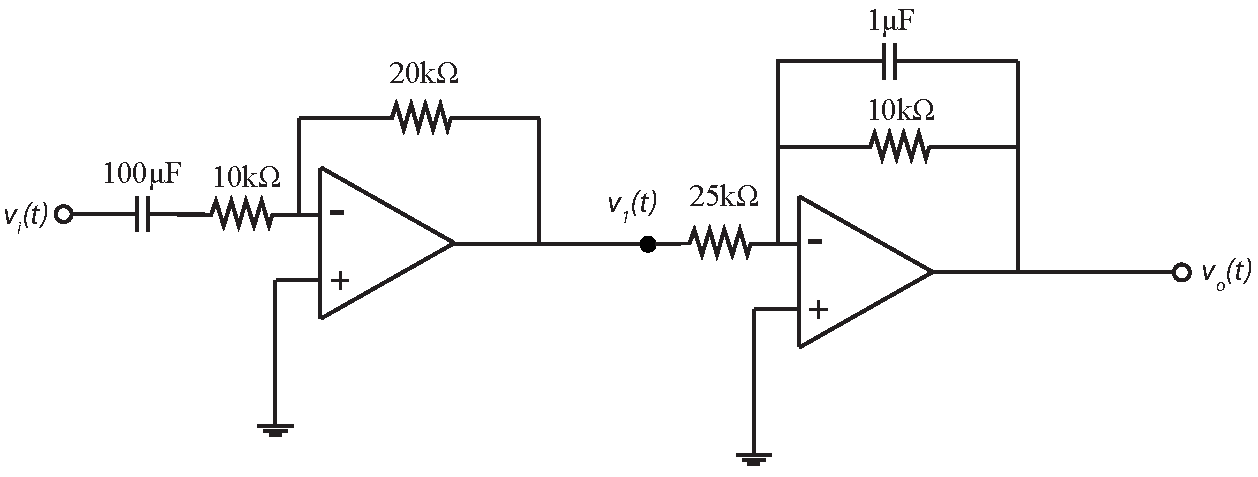
\includegraphics[width=0.75\textwidth]{bandpass}
    \end{center}
\end{minipage}

\begin{enumerate}
  \item Given that $u(t) = v_i(t)$ and $y(t) = v_o(t)$, compute the
    transferfunction for the given (ideal) OPAMP circuit

\textbf{Solution:}

First let's compute $V_1(s)/U(s)$ 
%
\begin{align*}
\frac{U(S)}{ \frac{10^4}{s} + 10^4 } &= \frac{-V_1(S)}{ 2 \, 10^4} 
\\
\frac{V_1(s)}{U(s)} &= \frac{-2 s}{s + 1}
\end{align*}
%
Now let's compute $Y(s)/V_1(s)$ 
%
\begin{align*}
\frac{V_1(s)}{ 2.5 10^4} &= -Y(s) \left( s 10^{-6} + 10^{-4} \right)
\\
\frac{V_1(s)}{ 2.5 10^4} &= -Y(s) \left( s + 100 \right) 10^{-6}
\\
\frac{Y(s)}{V_1(s)} &= \frac{-40}{s + 100}
\end{align*}
%
Hence, the transfer function of the whole system/circuit can be found
as
%
\begin{align*}
G(s) &= \frac{Y(s)}{U(s)} = \frac{Y(s)}{V_1(s)} \frac{V_1(s)}{U(s)}
\\
&= \frac{80 s}{(s + 100) (s+1)}
\\
&= \frac{80 s}{s^2 + 101 s + 100}
\end{align*}

\item Now find a state-space representation from the given TF.

\textbf{Solution:}

If we follow the derivation of controllable canonical form for a
second order system we obtain the following structure
%
\begin{align*}
	\dot{x} &= \left[ \begin{array}{cc} 0 & 1  \\  -a_0 & -a_1 \end{array} \right] x 
	+ \left[ \begin{array}{c} 0 \\ 1 \end{array} \right] u
	\\
	y &= \left[ \begin{array}{ccc} ( b_0 - b_2 a_0 ) & ( b_1 - b_2
                                                           a_1 )  \end{array} \right] x
	+ \left[ b_2 \right] u
\end{align*}
%
where 
%
\begin{align*}
a_0= 100 \ , \ a_1 = 101 \ , \ b_0 = 0 \ , \ b_1 = 80 \ ,\& \ b_2 = 0
\end{align*}
%
Thus, the state-space representation takes the form
%
\begin{align*}
	\dot{x} &= \left[ \begin{array}{cc} 0 & 1  \\  -100 & -101 \end{array} \right] x 
	+ \left[ \begin{array}{c} 0 \\ 1 \end{array} \right] u
	\\
	y &= \left[ \begin{array}{ccc} 0 & 80  \end{array} \right] x
\end{align*}
%

\item Now re-compute the TF from the given state-space representation

\textbf{Solution:}
%
\begin{align*}
G(s) &= C \left( s I - A \right)^{-1} B + D
\\
&= \left[ \begin{array}{ccc} 0 & 80  \end{array} \right]
                                 \left[ \begin{array}{cc} s & -1  \\
                                          100 & s+ 101 \end{array}
                                                \right]^{-1} \left[ \begin{array}{c} 0 \\ 1 \end{array} \right]
\\
&= \left[ \begin{array}{ccc} 0 & 80  \end{array} \right]
                                 \frac{1}{s^2+101 s + 100} 
\left[ \begin{array}{cc} s+101 & 1  \\ -100 & s \end{array} \right]
\left[ \begin{array}{c} 0 \\ 1 \end{array} \right]
\\
&= \left[ \begin{array}{ccc} 0 & 80  \end{array} \right]
\left[ \begin{array}{c} 1 \\ s \end{array} \right]
\frac{1}{s^2+101 s + 100} 
\\
&= \frac{80 s}{s^2+101 s + 100} 
\end{align*}

\end{enumerate}

\textbf{Take Home Problem:} 
\begin{enumerate}
\item First find state space representations of the
sub-system transfer functions, i.e. $\frac{V_1(s)}{U(s)}$ and
$\frac{Y(s)}{V_1(s)}$, separately.
\item Then combine the state-space
representations of the sub-systems to find a state-space representation 
for the whole system. 
\item Compute the TF from the computed state-space representation 
and compare it to the previous results.
\end{enumerate}

%

% **** This ENDS THE EXAMPLES. DON'T DELETE THE FOLLOWING LINE:
\end{document}
